% This file was created with tikzplotlib v0.10.1.
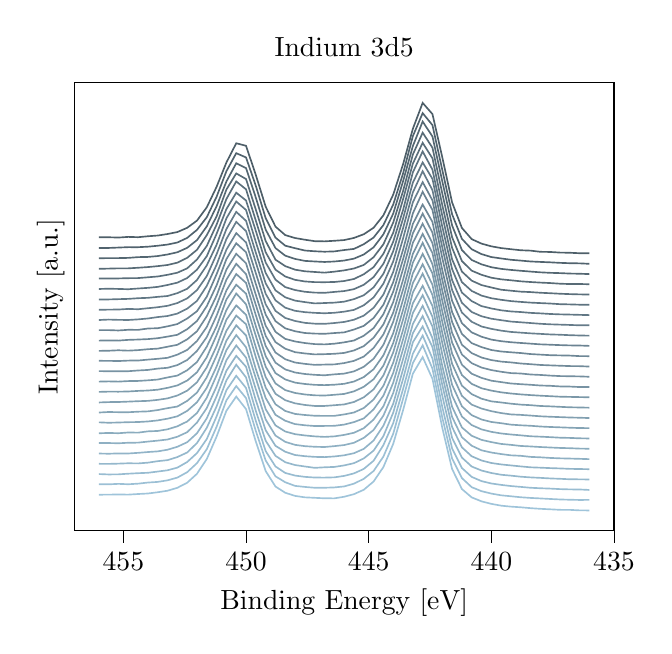
\begin{tikzpicture}

\definecolor{darkgray133164181}{RGB}{133,164,181}
\definecolor{darkgray136168186}{RGB}{136,168,186}
\definecolor{darkgray139172190}{RGB}{139,172,190}
\definecolor{darkgray143176195}{RGB}{143,176,195}
\definecolor{darkgray146180200}{RGB}{146,180,200}
\definecolor{darkgray176}{RGB}{176,176,176}
\definecolor{dimgray7895105}{RGB}{78,95,105}
\definecolor{dimgray8199110}{RGB}{81,99,110}
\definecolor{dimgray84103114}{RGB}{84,103,114}
\definecolor{dimgray88107118}{RGB}{88,107,118}
\definecolor{dimgray91111123}{RGB}{91,111,123}
\definecolor{lightslategray114139154}{RGB}{114,139,154}
\definecolor{lightslategray117143159}{RGB}{117,143,159}
\definecolor{lightslategray120147163}{RGB}{120,147,163}
\definecolor{lightslategray123152168}{RGB}{123,152,168}
\definecolor{lightslategray126156172}{RGB}{126,156,172}
\definecolor{lightslategray130160177}{RGB}{130,160,177}
\definecolor{lightsteelblue149184204}{RGB}{149,184,204}
\definecolor{lightsteelblue152188209}{RGB}{152,188,209}
\definecolor{lightsteelblue156192213}{RGB}{156,192,213}
\definecolor{lightsteelblue159196218}{RGB}{159,196,218}
\definecolor{slategray101123137}{RGB}{101,123,137}
\definecolor{slategray104127141}{RGB}{104,127,141}
\definecolor{slategray107131146}{RGB}{107,131,146}
\definecolor{slategray110135150}{RGB}{110,135,150}
\definecolor{slategray94115128}{RGB}{94,115,128}
\definecolor{slategray97119132}{RGB}{97,119,132}

\begin{axis}[
scaled y ticks=manual:{}{\pgfmathparse{#1}},
tick align=outside,
title={Indium 3d5},
x dir=reverse,
x grid style={darkgray176},
xlabel={Binding Energy [eV]},
xmin=435, xmax=457,
xtick pos=left,
xtick style={color=black},
y grid style={darkgray176},
ylabel={Intensity [a.u.]},
ymajorticks=false,
ymin=-132984.25, ymax=85129.25,
ytick style={color=black},
yticklabels={}
]
\addplot [semithick, dimgray7895105]
table {%
456 9868
455.6 9831
455.2 9693
454.8 10012
454.4 9863
454 10323
453.6 10671
453.2 11415
452.8 12358
452.4 14438
452 17936
451.6 24420
451.2 34391
450.8 46228
450.4 55572
450 54328
449.6 40045
449.2 24715
448.8 15013
448.4 10873
448 9454
447.6 8640
447.2 7932
446.8 7842
446.4 8125
446 8469
445.6 9509
445.2 11307
444.8 14451
444.4 20509
444 30575
443.6 45289
443.2 62594
442.8 75215
442.4 69743
442 48762
441.6 26794
441.2 14359
440.8 8914
440.4 6728
440 5422
439.6 4569
439.2 4020
438.8 3514
438.4 3328
438 2757
437.6 2681
437.2 2378
436.8 2295
436.4 2063
436 2019
};
\addplot [semithick, dimgray8199110]
table {%
456 4640
455.6 4636
455.2 4827
454.8 5015
454.4 5006
454 5243
453.6 5708
453.2 6283
452.8 7286
452.4 9531
452 13426
451.6 19599
451.2 29579
450.8 41982
450.4 50747
450 48652
449.6 34798
449.2 19109
448.8 9664
448.4 5716
448 4511
447.6 3382
447.2 3023
446.8 2802
446.4 2951
446 3618
445.6 4170
445.2 6461
444.8 9708
444.4 15765
444 25771
443.6 40841
443.2 59016
442.8 70241
442.4 64373
442 42612
441.6 21035
441.2 9065
440.8 3988
440.4 1643
440 200
439.6 -471
439.2 -1117
438.8 -1520
438.4 -1944
438 -2164
437.6 -2361
437.2 -2616
436.8 -2792
436.4 -2865
436 -3090
};
\addplot [semithick, dimgray84103114]
table {%
456 -396
455.6 -298
455.2 -301
454.8 -199
454.4 171
454 271
453.6 694
453.2 1461
452.8 2540
452.4 4687
452 8450
451.6 15155
451.2 24961
450.8 36990
450.4 45841
450 43479
449.6 29075
449.2 13545
448.8 4577
448.4 853
448 -704
447.6 -1661
447.2 -1941
446.8 -2187
446.4 -1957
446 -1490
445.6 -572
445.2 1458
444.8 4949
444.4 11269
444 21353
443.6 37023
443.2 54186
442.8 66117
442.4 58867
442 37061
441.6 15619
441.2 3614
440.8 -1225
440.4 -3338
440 -4738
439.6 -5545
439.2 -6059
438.8 -6473
438.4 -6862
438 -7228
437.6 -7470
437.2 -7608
436.8 -7824
436.4 -7914
436 -8086
};
\addplot [semithick, dimgray88107118]
table {%
456 -5519
455.6 -5414
455.2 -5290
454.8 -5286
454.4 -5004
454 -4668
453.6 -4212
453.2 -3651
452.8 -2524
452.4 -184
452 3727
451.6 10852
451.2 20015
450.8 33072
450.4 40900
450 38159
449.6 23244
449.2 8000
448.8 -1072
448.4 -4214
448 -5944
447.6 -6720
447.2 -7052
446.8 -7383
446.4 -6901
446 -6274
445.6 -5366
445.2 -3625
444.8 145
444.4 6430
444 16996
443.6 32296
443.2 50076
442.8 60721
442.4 53388
442 31178
441.6 9851
441.2 -1746
440.8 -6429
440.4 -8437
440 -9846
439.6 -10626
439.2 -11098
438.8 -11604
438.4 -11939
438 -12224
437.6 -12443
437.2 -12762
436.8 -12930
436.4 -12899
436 -13035
};
\addplot [semithick, dimgray91111123]
table {%
456 -10210
455.6 -10262
455.2 -10197
454.8 -10074
454.4 -10024
454 -9639
453.6 -9247
453.2 -8431
452.8 -7410
452.4 -5287
452 -991
451.6 5632
451.2 16031
450.8 28453
450.4 36995
450 33140
449.6 17884
449.2 2531
448.8 -5951
448.4 -9247
448 -10888
447.6 -11667
447.2 -11996
446.8 -12029
446.4 -11925
446 -11457
445.6 -10461
445.2 -8169
444.8 -4691
444.4 1817
444 12059
443.6 28262
443.2 45659
442.8 55781
442.4 48227
442 25470
441.6 4688
441.2 -6856
440.8 -11293
440.4 -13430
440 -14602
439.6 -15683
439.2 -16167
438.8 -16630
438.4 -16838
438 -17167
437.6 -17385
437.2 -17646
436.8 -17829
436.4 -17957
436 -18034
};
\addplot [semithick, slategray94115128]
table {%
456 -15326
455.6 -15200
455.2 -15306
454.8 -15447
454.4 -15097
454 -14776
453.6 -14311
453.2 -13378
452.8 -12255
452.4 -9999
452 -5924
451.6 659
451.2 11507
450.8 23570
450.4 31519
450 27723
449.6 12881
449.2 -2467
448.8 -10807
448.4 -14432
448 -15846
447.6 -16690
447.2 -17094
446.8 -17206
446.4 -16754
446 -16342
445.6 -15406
445.2 -13281
444.8 -9539
444.4 -3052
444 7680
443.6 23075
443.2 41393
442.8 51585
442.4 42723
442 20362
441.6 -898
441.2 -11991
440.8 -16283
440.4 -18553
440 -19835
439.6 -20594
439.2 -21226
438.8 -21613
438.4 -21965
438 -22187
437.6 -22404
437.2 -22722
436.8 -22830
436.4 -22975
436 -23017
};
\addplot [semithick, slategray97119132]
table {%
456 -20476
455.6 -20414
455.2 -20280
454.8 -20143
454.4 -19817
454 -19632
453.6 -19157
453.2 -18749
452.8 -17346
452.4 -15241
452 -10959
451.6 -3811
451.2 6239
450.8 19045
450.4 27242
450 23087
449.6 7488
449.2 -7552
448.8 -16008
448.4 -19400
448 -20994
447.6 -21711
447.2 -22344
446.8 -22162
446.4 -21969
446 -21492
445.6 -20263
445.2 -18376
444.8 -14532
444.4 -7925
444 3056
443.6 18904
443.2 36416
442.8 46256
442.4 38212
442 14989
441.6 -5651
441.2 -17083
440.8 -21235
440.4 -23663
440 -24797
439.6 -25700
439.2 -26252
438.8 -26546
438.4 -26955
438 -27194
437.6 -27491
437.2 -27673
436.8 -27781
436.4 -27918
436 -28038
};
\addplot [semithick, slategray101123137]
table {%
456 -25473
455.6 -25369
455.2 -25327
454.8 -25023
454.4 -25184
454 -24695
453.6 -24206
453.2 -23521
452.8 -22163
452.4 -19906
452 -15880
451.6 -9032
451.2 1596
450.8 13847
450.4 22200
450 17824
449.6 2272
449.2 -12593
448.8 -20855
448.4 -24452
448 -25955
447.6 -26602
447.2 -26943
446.8 -27135
446.4 -26913
446 -26364
445.6 -25498
445.2 -23253
444.8 -19421
444.4 -12735
444 -1934
443.6 14185
443.2 31629
442.8 41974
442.4 32744
442 9763
441.6 -10998
441.2 -22047
440.8 -26535
440.4 -28604
440 -29782
439.6 -30509
439.2 -31183
438.8 -31531
438.4 -31898
438 -32263
437.6 -32514
437.2 -32673
436.8 -32825
436.4 -33004
436 -33010
};
\addplot [semithick, slategray104127141]
table {%
456 -30428
455.6 -30212
455.2 -30356
454.8 -30408
454.4 -30115
454 -29681
453.6 -28999
453.2 -28473
452.8 -27299
452.4 -24921
452 -21120
451.6 -13787
451.2 -3525
450.8 9002
450.4 17327
450 12828
449.6 -2452
449.2 -17667
448.8 -25991
448.4 -29437
448 -30895
447.6 -31816
447.2 -32203
446.8 -32286
446.4 -31889
446 -31371
445.6 -30282
445.2 -28297
444.8 -24482
444.4 -18028
444 -7030
443.6 9166
443.2 26849
442.8 36673
442.4 27793
442 4889
441.6 -15833
441.2 -26789
440.8 -31299
440.4 -33580
440 -34725
439.6 -35592
439.2 -36219
438.8 -36572
438.4 -36913
438 -37168
437.6 -37439
437.2 -37586
436.8 -37809
436.4 -37950
436 -38043
};
\addplot [semithick, slategray107131146]
table {%
456 -35368
455.6 -35345
455.2 -35512
454.8 -35183
454.4 -35220
454 -34558
453.6 -34421
453.2 -33504
452.8 -32382
452.4 -29713
452 -26143
451.6 -19046
451.2 -8124
450.8 3838
450.4 11839
450 7316
449.6 -7705
449.2 -22791
448.8 -30978
448.4 -34486
448 -35891
447.6 -36752
447.2 -37032
446.8 -37135
446.4 -36762
446 -36438
445.6 -35051
445.2 -33271
444.8 -29448
444.4 -22971
444 -11997
443.6 3755
443.2 21474
442.8 31927
442.4 23121
442 -231
441.6 -21075
441.2 -31961
440.8 -36452
440.4 -38557
440 -39959
439.6 -40726
439.2 -41233
438.8 -41588
438.4 -41921
438 -42264
437.6 -42447
437.2 -42636
436.8 -42777
436.4 -42839
436 -43010
};
\addplot [semithick, slategray110135150]
table {%
456 -40441
455.6 -40376
455.2 -40435
454.8 -40087
454.4 -39923
454 -39709
453.6 -39282
453.2 -38492
452.8 -37620
452.4 -34898
452 -30901
451.6 -23671
451.2 -13473
450.8 -773
450.4 6915
450 2551
449.6 -12953
449.2 -27803
448.8 -36172
448.4 -39617
448 -40860
447.6 -41631
447.2 -42141
446.8 -42284
446.4 -41947
446 -41290
445.6 -40394
445.2 -38065
444.8 -34365
444.4 -27567
444 -16654
443.6 -921
443.2 16330
442.8 25753
442.4 17303
442 -6125
441.6 -26556
441.2 -37180
440.8 -41672
440.4 -43615
440 -45011
439.6 -45741
439.2 -46125
438.8 -46491
438.4 -46988
438 -47262
437.6 -47534
437.2 -47641
436.8 -47731
436.4 -47991
436 -48025
};
\addplot [semithick, lightslategray114139154]
table {%
456 -45439
455.6 -45365
455.2 -45148
454.8 -45334
454.4 -45080
454 -44631
453.6 -44349
453.2 -43416
452.8 -42484
452.4 -39830
452 -35905
451.6 -28547
451.2 -18530
450.8 -5858
450.4 1820
450 -2838
449.6 -18209
449.2 -33214
448.8 -41190
448.4 -44387
448 -46077
447.6 -46687
447.2 -47149
446.8 -47039
446.4 -46861
446 -46437
445.6 -45233
445.2 -43126
444.8 -39036
444.4 -32548
444 -21716
443.6 -5639
443.2 11766
442.8 21357
442.4 12048
442 -10924
441.6 -31396
441.2 -42446
440.8 -46534
440.4 -48674
440 -49917
439.6 -50649
439.2 -51052
438.8 -51580
438.4 -51917
438 -52288
437.6 -52490
437.2 -52670
436.8 -52835
436.4 -52883
436 -53073
};
\addplot [semithick, lightslategray117143159]
table {%
456 -50281
455.6 -50288
455.2 -50386
454.8 -50165
454.4 -50134
454 -49697
453.6 -49295
453.2 -48815
452.8 -47283
452.4 -44986
452 -40637
451.6 -33777
451.2 -23199
450.8 -10790
450.4 -3053
450 -8123
449.6 -23146
449.2 -38141
448.8 -46247
448.4 -49510
448 -51108
447.6 -51763
447.2 -52247
446.8 -52112
446.4 -52019
446 -51376
445.6 -50292
445.2 -48218
444.8 -44022
444.4 -37420
444 -26819
443.6 -10911
443.2 7099
442.8 16432
442.4 6936
442 -16088
441.6 -36674
441.2 -47191
440.8 -51427
440.4 -53555
440 -54781
439.6 -55605
439.2 -56253
438.8 -56444
438.4 -56926
438 -57147
437.6 -57468
437.2 -57703
436.8 -57778
436.4 -57865
436 -58032
};
\addplot [semithick, lightslategray120147163]
table {%
456 -55276
455.6 -55364
455.2 -55378
454.8 -55323
454.4 -54980
454 -54713
453.6 -54062
453.2 -53674
452.8 -52358
452.4 -49886
452 -45475
451.6 -38711
451.2 -28283
450.8 -16010
450.4 -8049
450 -12384
449.6 -28150
449.2 -43044
448.8 -51188
448.4 -54470
448 -55957
447.6 -56692
447.2 -57092
446.8 -57315
446.4 -56863
446 -56505
445.6 -55408
445.2 -53182
444.8 -49269
444.4 -42479
444 -31303
443.6 -15645
443.2 1782
442.8 11463
442.4 2159
442 -21033
441.6 -41390
441.2 -52155
440.8 -56568
440.4 -58577
440 -59943
439.6 -60620
439.2 -61308
438.8 -61639
438.4 -61939
438 -62287
437.6 -62438
437.2 -62735
436.8 -62807
436.4 -63033
436 -63015
};
\addplot [semithick, lightslategray123152168]
table {%
456 -60391
455.6 -60288
455.2 -60392
454.8 -60137
454.4 -60057
454 -59771
453.6 -59389
453.2 -58362
452.8 -57458
452.4 -54878
452 -50855
451.6 -43355
451.2 -33451
450.8 -20396
450.4 -13254
450 -17607
449.6 -33448
449.2 -47992
448.8 -56270
448.4 -59337
448 -60894
447.6 -61550
447.2 -61962
446.8 -62100
446.4 -61900
446 -61458
445.6 -60353
445.2 -58180
444.8 -54360
444.4 -47588
444 -36834
443.6 -20501
443.2 -2545
442.8 7136
442.4 -3261
442 -26209
441.6 -46757
441.2 -57191
440.8 -61502
440.4 -63625
440 -64769
439.6 -65606
439.2 -66178
438.8 -66611
438.4 -66952
438 -67243
437.6 -67480
437.2 -67732
436.8 -67826
436.4 -67928
436 -68017
};
\addplot [semithick, lightslategray126156172]
table {%
456 -65402
455.6 -65259
455.2 -65292
454.8 -65196
454.4 -64911
454 -64721
453.6 -64326
453.2 -63427
452.8 -62246
452.4 -59899
452 -55857
451.6 -48503
451.2 -37756
450.8 -25567
450.4 -17514
450 -22766
449.6 -38167
449.2 -53113
448.8 -61290
448.4 -64536
448 -65918
447.6 -66650
447.2 -67061
446.8 -67171
446.4 -66805
446 -66384
445.6 -65130
445.2 -62915
444.8 -59238
444.4 -52593
444 -41616
443.6 -25549
443.2 -7648
442.8 1738
442.4 -7817
442 -31298
441.6 -51736
441.2 -62347
440.8 -66487
440.4 -68706
440 -69995
439.6 -70537
439.2 -71128
438.8 -71586
438.4 -71853
438 -72245
437.6 -72433
437.2 -72667
436.8 -72880
436.4 -72977
436 -73080
};
\addplot [semithick, lightslategray130160177]
table {%
456 -70535
455.6 -70358
455.2 -70307
454.8 -70127
454.4 -69920
454 -69763
453.6 -69273
453.2 -68553
452.8 -67149
452.4 -64816
452 -60723
451.6 -53436
451.2 -43083
450.8 -30257
450.4 -23323
450 -27897
449.6 -43668
449.2 -58188
448.8 -66312
448.4 -69452
448 -70964
447.6 -71761
447.2 -72231
446.8 -72235
446.4 -71882
446 -71495
445.6 -70295
445.2 -68029
444.8 -64156
444.4 -57352
444 -46200
443.6 -30242
443.2 -12469
442.8 -3291
442.4 -13314
442 -36638
441.6 -56824
441.2 -67308
440.8 -71595
440.4 -73504
440 -74775
439.6 -75698
439.2 -76350
438.8 -76578
438.4 -76907
438 -77271
437.6 -77489
437.2 -77664
436.8 -77850
436.4 -77965
436 -78126
};
\addplot [semithick, darkgray133164181]
table {%
456 -75436
455.6 -75177
455.2 -75269
454.8 -75280
454.4 -75030
454 -74874
453.6 -74240
453.2 -73306
452.8 -72513
452.4 -69778
452 -65743
451.6 -58284
451.2 -47692
450.8 -35626
450.4 -28274
450 -32480
449.6 -48518
449.2 -63291
448.8 -71423
448.4 -74681
448 -76119
447.6 -76634
447.2 -77003
446.8 -77078
446.4 -77047
446 -76354
445.6 -75412
445.2 -73236
444.8 -69089
444.4 -62424
444 -51172
443.6 -35276
443.2 -17054
442.8 -7911
442.4 -18228
442 -41617
441.6 -61934
441.2 -72392
440.8 -76716
440.4 -78834
440 -80016
439.6 -80629
439.2 -81331
438.8 -81647
438.4 -81877
438 -82239
437.6 -82465
437.2 -82640
436.8 -82822
436.4 -82984
436 -83022
};
\addplot [semithick, darkgray136168186]
table {%
456 -80204
455.6 -80409
455.2 -80289
454.8 -80137
454.4 -80057
454 -79778
453.6 -79266
453.2 -78421
452.8 -77276
452.4 -74640
452 -70429
451.6 -63389
451.2 -53022
450.8 -40437
450.4 -33025
450 -37934
449.6 -54332
449.2 -68366
448.8 -76554
448.4 -79460
448 -81057
447.6 -81638
447.2 -81998
446.8 -81949
446.4 -81899
446 -81301
445.6 -80095
445.2 -78278
444.8 -73885
444.4 -67202
444 -56140
443.6 -39892
443.2 -22267
442.8 -13816
442.4 -23566
442 -47244
441.6 -67121
441.2 -77368
440.8 -81539
440.4 -83639
440 -84833
439.6 -85618
439.2 -86119
438.8 -86537
438.4 -86984
438 -87180
437.6 -87409
437.2 -87677
436.8 -87785
436.4 -87976
436 -88060
};
\addplot [semithick, darkgray139172190]
table {%
456 -85525
455.6 -85371
455.2 -85503
454.8 -85142
454.4 -85219
454 -84591
453.6 -84403
453.2 -83591
452.8 -82136
452.4 -79797
452 -75664
451.6 -68197
451.2 -57311
450.8 -45065
450.4 -37732
450 -43693
449.6 -58792
449.2 -73810
448.8 -81701
448.4 -84670
448 -85970
447.6 -86583
447.2 -87036
446.8 -87291
446.4 -87035
446 -86326
445.6 -85276
445.2 -83061
444.8 -78854
444.4 -72405
444 -60946
443.6 -44657
443.2 -27027
442.8 -18343
442.4 -28882
442 -52756
441.6 -72613
441.2 -82693
440.8 -86749
440.4 -88741
440 -89818
439.6 -90709
439.2 -91162
438.8 -91698
438.4 -91935
438 -92214
437.6 -92444
437.2 -92662
436.8 -92788
436.4 -92982
436 -93049
};
\addplot [semithick, darkgray143176195]
table {%
456 -90287
455.6 -90278
455.2 -90388
454.8 -90144
454.4 -90085
454 -89566
453.6 -89108
453.2 -88558
452.8 -87209
452.4 -85004
452 -80335
451.6 -73209
451.2 -62730
450.8 -49992
450.4 -42782
450 -48717
449.6 -64160
449.2 -78817
448.8 -86655
448.4 -89709
448 -91166
447.6 -91800
447.2 -92094
446.8 -92215
446.4 -91788
446 -91260
445.6 -90151
445.2 -87779
444.8 -83909
444.4 -76928
444 -65954
443.6 -49497
443.2 -32343
442.8 -23533
442.4 -33570
442 -57409
441.6 -77565
441.2 -87445
440.8 -91591
440.4 -93813
440 -94891
439.6 -95638
439.2 -96262
438.8 -96492
438.4 -97021
438 -97218
437.6 -97526
437.2 -97716
436.8 -97828
436.4 -97961
436 -98120
};
\addplot [semithick, darkgray146180200]
table {%
456 -95380
455.6 -95479
455.2 -95330
454.8 -95362
454.4 -95049
454 -94656
453.6 -94334
453.2 -93527
452.8 -92093
452.4 -89884
452 -85522
451.6 -78225
451.2 -67507
450.8 -55087
450.4 -47841
450 -53169
449.6 -69512
449.2 -84045
448.8 -91642
448.4 -94528
448 -96105
447.6 -96678
447.2 -97010
446.8 -97118
446.4 -96808
446 -96241
445.6 -95220
445.2 -93109
444.8 -89037
444.4 -81822
444 -71125
443.6 -54447
443.2 -36844
442.8 -28501
442.4 -39245
442 -61999
441.6 -82445
441.2 -92374
440.8 -96722
440.4 -98761
440 -99985
439.6 -100684
439.2 -101168
438.8 -101651
438.4 -102088
438 -102267
437.6 -102475
437.2 -102631
436.8 -102834
436.4 -102920
436 -103014
};
\addplot [semithick, lightsteelblue149184204]
table {%
456 -100389
455.6 -100422
455.2 -100299
454.8 -100119
454.4 -100194
454 -99821
453.6 -99102
453.2 -98600
452.8 -97094
452.4 -94876
452 -90277
451.6 -82837
451.2 -72431
450.8 -59756
450.4 -52147
450 -58353
449.6 -74678
449.2 -89158
448.8 -96509
448.4 -99620
448 -100987
447.6 -101682
447.2 -102342
446.8 -102079
446.4 -101900
446 -101161
445.6 -100073
445.2 -97766
444.8 -93955
444.4 -86876
444 -75509
443.6 -59169
443.2 -41268
442.8 -33541
442.4 -43615
442 -67245
441.6 -87739
441.2 -97355
440.8 -101706
440.4 -103653
440 -104845
439.6 -105705
439.2 -106143
438.8 -106655
438.4 -106992
438 -107223
437.6 -107496
437.2 -107676
436.8 -107905
436.4 -107942
436 -108010
};
\addplot [semithick, lightsteelblue152188209]
table {%
456 -105372
455.6 -105560
455.2 -105506
454.8 -105195
454.4 -104945
454 -104752
453.6 -104144
453.2 -103527
452.8 -102240
452.4 -99515
452 -95168
451.6 -88316
451.2 -77289
450.8 -64558
450.4 -57550
450 -63495
449.6 -79556
449.2 -94184
448.8 -101689
448.4 -104833
448 -106111
447.6 -106736
447.2 -107067
446.8 -107093
446.4 -106973
446 -106268
445.6 -105045
445.2 -102866
444.8 -98890
444.4 -91281
444 -80594
443.6 -64065
443.2 -46796
442.8 -37961
442.4 -49165
442 -72728
441.6 -92863
441.2 -102430
440.8 -106751
440.4 -108804
440 -109960
439.6 -110640
439.2 -111205
438.8 -111612
438.4 -112043
438 -112269
437.6 -112440
437.2 -112694
436.8 -112832
436.4 -112872
436 -113106
};
\addplot [semithick, lightsteelblue156192213]
table {%
456 -110341
455.6 -110361
455.2 -110136
454.8 -110328
454.4 -110039
454 -109505
453.6 -109184
453.2 -108416
452.8 -107089
452.4 -104474
452 -100052
451.6 -93253
451.2 -82322
450.8 -69487
450.4 -62556
450 -68410
449.6 -84489
449.2 -98757
448.8 -106462
448.4 -109368
448 -111125
447.6 -111631
447.2 -112035
446.8 -112031
446.4 -111870
446 -111393
445.6 -110039
445.2 -107689
444.8 -103887
444.4 -96864
444 -85739
443.6 -68824
443.2 -51378
442.8 -42747
442.4 -54104
442 -77849
441.6 -97822
441.2 -107333
440.8 -111768
440.4 -113698
440 -114871
439.6 -115707
439.2 -116180
438.8 -116655
438.4 -116984
438 -117225
437.6 -117487
437.2 -117730
436.8 -117862
436.4 -117968
436 -117927
};
\addplot [semithick, lightsteelblue159196218]
table {%
456 -115412
455.6 -115375
455.2 -115312
454.8 -115372
454.4 -115074
454 -114829
453.6 -114217
453.2 -113476
452.8 -112047
452.4 -109587
452 -105229
451.6 -98032
451.2 -87114
450.8 -74555
450.4 -67657
450 -73770
449.6 -89597
449.2 -103928
448.8 -111437
448.4 -114476
448 -115994
447.6 -116698
447.2 -116931
446.8 -117160
446.4 -117185
446 -116406
445.6 -115154
445.2 -113011
444.8 -108989
444.4 -101965
444 -90662
443.6 -74365
443.2 -56535
442.8 -48445
442.4 -59040
442 -82858
441.6 -102894
441.2 -112649
440.8 -116735
440.4 -118648
440 -119872
439.6 -120745
439.2 -121217
438.8 -121535
438.4 -121959
438 -122283
437.6 -122518
437.2 -122771
436.8 -122793
436.4 -123036
436 -123070
};
\end{axis}

\end{tikzpicture}
